\section{Experimental Analysis}
\label{sec:evaluation}
Now we present an empirical evaluation of the effectiveness of our algorithm in solving the \sygurl problem. We synthesize programs for two \torcs tracks, CG-Speedway-1 and Aalborg. These tracks provide varying levels of difficulty, with Aalborg being the more difficult track of the two.

\subsection{Evaluating Performance}
A controller's performance is measured according to two metrics, \textit{lap time} and \textit{reward}. To calculate the lap time, the programs are allowed to complete a three lap race, and we report the average time taken to complete a lap during this race. The reward function is calculated using the car's velocity, angle with the track axis, and distance from the track axis. The same function is used to train the DRL agent initially. In the experiments we compare the average reward per time step, obtained by the various programs. 

We compare among the following \rl agents:
\begin{enumerate}[label=A\arabic*:]
	\item \textsc{DRL}. An agent which uses \drl to find a policy
	represented as a deep neural
	network. The specific \drl algorithm we use is Deep
	Deterministic Policy Gradients~\citep{ddpg}, which has
	previously been used on \torcs.  
	\item $\textit{Naive}$. Program synthesized without access to a policy oracle. 
	\item $\textit{NoAug}$. Program synthesized without input augmentation.
	\item $\textit{NoSketch}$. Program synthesized in our policy language without sketch guidance.
	\item $\textit{NoIF}$. Programs permitted by a restriction of
          our sketch that does not permit conditional branching.
	\item \algo. The Program generated by the \algo algorithm.
\end{enumerate}

In Table~\ref{table:performance} we present the performance results of the above list. The lap times in that table are given in minutes and seconds. The \textsc{Timeout} entries indicate that the synthesis process did not return a program that could complete the race, within the specified timeout of twelve hours.

These results justify the various choices that we made in our \algo algorithm architecture, as discussed in Section~\ref{sec:algorithm}. In many cases those choices were necessary to be able to synthesize a program that could successfully complete a race. As a consequence of these results, we only consider the DRL agent and the \algo program for subsequent comparisons.

The $\textit{NoAug}$ and $\textit{NoSketch}$ agents are unable to
generate programs that complete a single lap on either track. In the
case of $\textit{NoSketch}$ this is because the syntax of the policy
language (Figure~\ref{fig:syntax}), defines a very large program
space. If we randomly sample from this space without any constraints
(like those provided by the sketch), then the probability of getting a
good program is extremely low and hence we are unable to reliably
generate a program that can complete a lap. The $\textit{NoAug}$ agent
performs poorly because without input augmentation, the synthesizer
has no guidance from the oracle regarding the ``correct'' behavior once the program deviates even slightly from the oracle's trajectory.

The \algo algorithm is biased towards generating simpler programs to aid in interpretability. In the \algo algorithm experiments we allow the synthesizer to produce policies with up to five nested $\ifc$ statements. However, if two policies have \textsc{Lap Times} within one second of each other, then the algorithm chooses the one with fewer $\ifc$ statements as the output. This is a reasonable choice because a difference of less than one second in \textsc{Lap Times} can be the result of different starting positions in the \torcs simulator, and hence the performance of such policies is essentially equivalent.

\begin{table}[h]
	\caption{Performance results in \torcs. Lap time is given in Minutes:Seconds. Timeout indicates that the synthesizer did not return a program that completed the race within the specified timeout.}
	\label{table:performance}
	\begin{center}
		\begin{small}
			\begin{sc}
				\begin{tabular}{l c c cc}
					\toprule
					Model &  \multicolumn{2}{ c }{CG-Speedway-1} &  \multicolumn{2}{ c }{Aalborg}  \\
					%\vskip 1pt
					\cline{2-5}
					& Lap Time & Reward  & Lap Time & Reward   \\
					\midrule					
					Drl & 54.27 & 118.39 & 1:49.66 &  71.23  \\
					$\textit{Naive}$  &  2:07.09 & 58.72 & Timeout  & $-$\\
					$\textit{NoAug}$  & Timeout  & $-$ & Timeout  & $-$\\
					$\textit{NoSketch}$ & Timeout  & $-$ & Timeout  & $-$\\
					$\textit{NoIF}$ & 1:01.60  & 115.25 & 2:45.13  & 52.81  \\
					\algo & 1:01.56 & 115.32 &  2:38.87 & 54.91\\	
					\bottomrule
				\end{tabular}
			\end{sc}
		\end{small}
	\end{center}
\end{table}

\subsection{Qualitative Analysis of the Programmatic Policy}
We provide qualitative analysis of the inferred programmatic policy through the lens of interpretability, and its behavior in acting in the environment.

\paragraph{Interpretability.} 
Interpretability is a qualitative metric, and cannot be easily
demonstrated via  experiments. The \drl policies are considered uninterpretable because their policies
are encoded in black box neural networks. 
In contrast, the \pirl policies are compact and
human-readable by construction, as
exemplified by the acceleration policy in Figure~\ref{fig:code}. More examples of our synthesized policies are given in Appendix~\ref{sec:examples}.

\paragraph{Behavior of Policy.}
Our experimental validation showed that the programmatic policy was less aggressive in terms of its use of actions and resulting in smoother steering actions. Numerically, we measure smoothness in Table~\ref{table:smoothness} by comparing the population standard deviation of the set of steering actions taken by the program during the entire race. In Figure~\ref{fig:smoothness} we present a scatter plot of the steering actions taken by the DRL agent and the \algo program during a slice of the CG-Speedway-1 race. As we can see, the \algo program takes much more conservative actions.

\begin{figure}[t]
	\vspace{-0.1in}
	\begin{center}
		\centerline{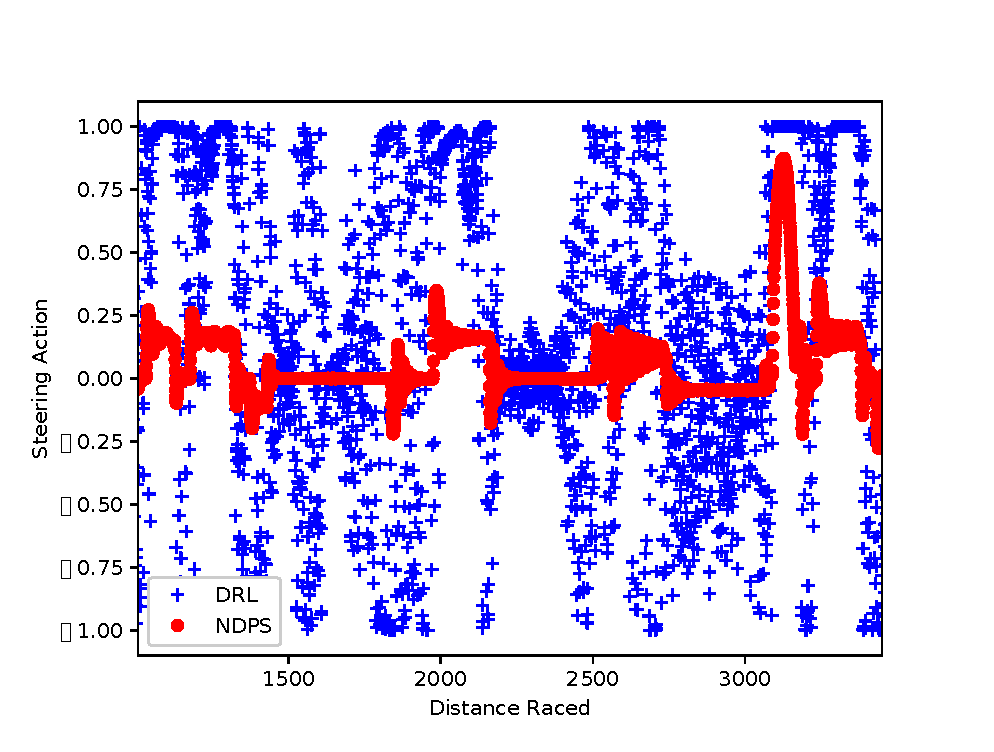
\includegraphics[scale=0.4]{steer_actions_scattern}}
		\caption{Slice of steering actions taken by the DRL and \algo agents, during the CG-Speedway-1 race. This figure demonstrates that the \algo agent drives more smoothly.}
		\label{fig:smoothness}
	\end{center}
	\vspace{-0.2in}
\end{figure}

\begin{table}[h]
	\caption{Smoothness measure of agents in \torcs, given by the standard deviation of the steering actions during a complete race. Lower values indicate smoother steering.}
	\label{table:smoothness}
	\begin{center}
		\begin{small}
			\begin{sc}
				\begin{tabular}{l c c }
					\toprule
					Model &  CG-Speedway-1 & Aalborg  \\ 
					\midrule
					Drl & 0.5981  & 0.9008  \\
					\algo & 0.1312 & 0.2483  \\					
					\bottomrule
				\end{tabular}
			\end{sc}
		\end{small}
	\end{center}
\end{table}

\subsection{Robustness to Missing/Noisy Features}
To evaluate the robustness of the agents with respect to defective sensors we introduce a \emph{Partial Observability} variant of \torcs. In this variant, a random sample of $j$ sensors are declared defective. During the race, one or more of these defective sensors are blocked with some fixed probability. Hence, during game-play, the sensor either returns the correct reading or a \emph{null} reading. For sufficiently high block probabilities, both agents will fail to complete the race. In Table~\ref{table:partial} we show the distances raced for two values of the block probability, and in Figure~\ref{fig:partial} we plot the distance raced as we increase the block probability on the Aalborg track. In both these experiments, the set of defective sensors was taken to be $\{\rpm, \tangle\}$ because we know that the synthesized programs crucially depend on these sensors.

\begin{table}[h]
	\caption{Partial observability results in \torcs blocking sensors $\{\rpm, \tangle\}$ . For each track and block probability we give the distance, in meters, raced by the program before crashing.}
	\label{table:partial}
	\begin{center}
		\begin{small}
			\begin{sc}
				\begin{tabular}{l c c cc}
					\toprule
					Model &  \multicolumn{2}{ c }{CG-Speedway-1} &  \multicolumn{2}{ c }{Aalborg}  \\ 
					\cline{2-5}
					& 50\% & 90\%  & 50\% & 90\%     \\
					\midrule				
					Drl & 21 & 17 & 71 &  20  \\					
					\algo & 1976 & 200 &  1477	 & 287\\
					\bottomrule
				\end{tabular}
			\end{sc}
		\end{small}
	\end{center}
\end{table}

\begin{figure}[h]
	\vskip -0.11in
	\begin{center}
		\centerline{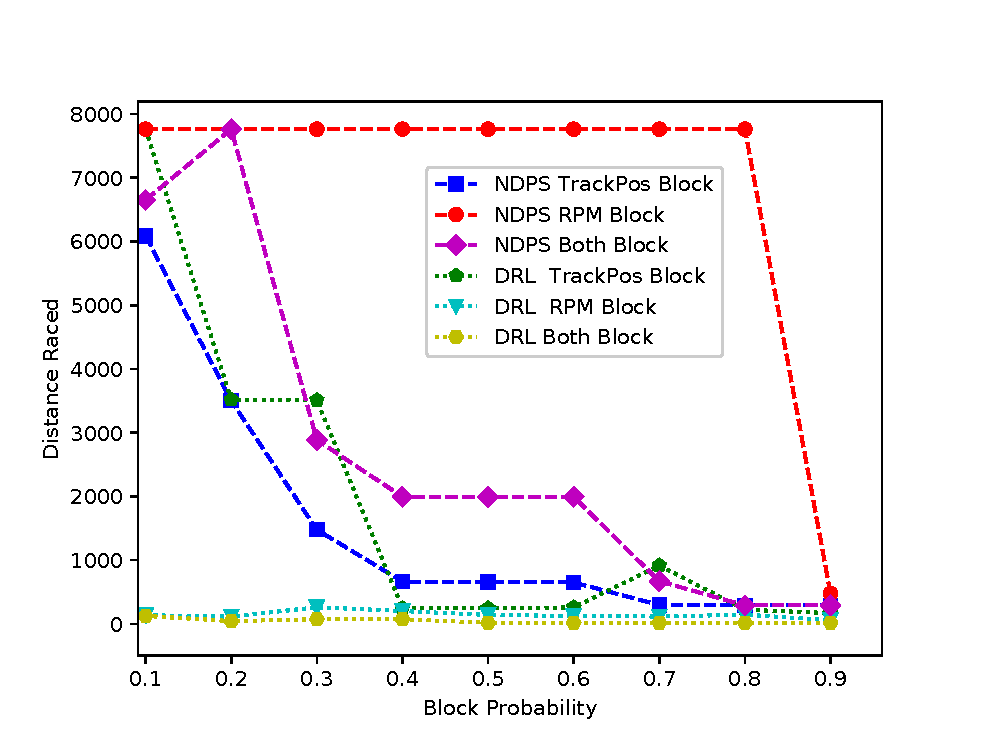
\includegraphics[width=\columnwidth]{po_3allblock}}
		\caption{Distance raced by the agents as the block probability increases for a particular sensor(s) on Aalborg. The \algo agent is more robust to blocked sensors.}
		\label{fig:partial}
	\end{center}
	\vskip -0.2in
\end{figure}


\subsection{Evaluating Generalization to New Instances}
To compare the ability of the agents to perform on unseen tracks, we executed the learned policies on tracks of comparable difficulty. For agents trained on the CG-Speedway-1 track, we chose CG track 2 and E-Road as the transfer tracks, and for Aalborg trained tracks we chose Alpine 2 and Ruudskogen. As can be seen in Tables \ref{table:cgspeed} and \ref{table:aalborg}, the \algo programmatically synthesized program far outperforms the DRL agent on unseen tracks. The DRL agent is unable to complete the race on any of these transfer tracks. This demonstrates the transferability of the policies \algo finds.


\begin{table}[h]
	\caption{Transfer results with training on CG-Speedway-1. `Cr'
		indicates that the agent crashed after racing the specified distance.}
	\label{table:cgspeed}
	%	\vskip 0.15in
	\begin{center}
		\begin{small}
			\begin{sc}
				\begin{tabular}{l c c c c}
					\toprule
					Model &  \multicolumn{2}{ c }{CG track 2}  &  \multicolumn{2}{ c }{E-Road}   \\ 
					\cline{2-5}
					& Lap Time & Reward & Lap Time & Reward   \\
					\midrule					
					DRL &  Cr 1608m & $-$&  Cr 1902m & $-$ \\					
					\algo & 1:40.57 & 110.18 & 1:51.59 & 98.21 \\					
					\bottomrule
				\end{tabular}
			\end{sc}
		\end{small}
	\end{center}
	\caption{Transfer results with training on Aalborg. `Cr' denotes the agent crashed, after racing the specified distance.}
	\label{table:aalborg}
	\begin{center}
		\begin{small}
			\begin{sc}
				\begin{tabular}{l c c c c }
					\toprule
					Model &  \multicolumn{2}{ c }{Alpine 2}  &  \multicolumn{2}{ c }{Ruudskogen}   \\ 
					\cline{2-5}
					& Lap Time & Reward & Lap Time & Reward   \\
					\midrule					
					DRL &   Cr 1688m  & $-$&  Cr 3232m & $-$ \\					
					\algo & 3:16.68 &  67.49 & 3:19.77 & 57.69 \\										
					\bottomrule
				\end{tabular}
			\end{sc}
		\end{small}
	\end{center}
	\vspace{-0.2in}
\end{table}

\subsection{Verifiability of Policies}
Now we use established symbolic verification techniques to automatically prove two properties of policies generated by \algo. So far as we know, the current state of the art neural network verifiers cannot verify the DRL network we are using in a reasonable amount of time, due to the size and complexity of the network used to implement the DDPG algorithm. For example, the Reluplex~\cite{reluplex} algorithm was tested on networks at most 300 nodes wide, whereas our network has three layers with 600 nodes each, and other smaller layers.

\paragraph{Smoothness Property} For the program given in Figure~\ref{fig:code} we proved, we have $  \forall k, \ \sum_{i=k}^{k+5}\norm{\pickc(h_\rpm, i+1) - \pickc(h_\rpm, i)} < 0.006  \implies  \norm{\pickc(h_{\mathtt{Accel}}, k+1) - \pickc(h_{\mathtt{Accel}}, k)} < 0.49 $. Intuitively, the above logical implication means that if the sum of the consecutive differences of the last six $\rpm$ sensor values is less than $0.006$, then the acceleration actions calculated at the last and penultimate step will not differ by more than $0.49$. Similarly, for a policy given in Appendix~\ref{sec:examples}, we prove $  \forall k, \; \sum_{i=k}^{k+5}\norm{\pickc(h_\tangle, i+1) - \pickc(h_\tangle, i)} < 0.006 \implies \norm{\pickc(h_{\mathtt{Steer}}, k+1) - \pickc(h_{\mathtt{Steer}}, k)} < 0.11$. This proof gives us a guarantee of the type of smooth steering behavior that we empirically examined earlier in this section. 

\paragraph{Universal Bounds} We can prove that the program in Figure~\ref{fig:code} satisfies the property $  \forall i \; (0 \leq \pickc(h_\rpm, i) \leq 1 \wedge -1 \leq \pickc(h_\tangle, i) \leq 1) \implies (\norm{\pickc(h_\mathtt{Steer}, i)} < 101.08 \wedge -54.53 < \pickc(h_\mathtt{Accel}, i) < 53.03)$.  Intuitively, this means that we have proved global bounds for the action values in this environment, assuming reasonable bounds on some of the input values. In the \torcs environment these bounds are not very useful, since the simulator clips these actions to certain pre-specified ranges. However, this experiment demonstrates that our framework allows us to prove universal bounds on the actions, and this could be a critical property for other environments.